\chapter{Network Layer\label{chap:networklayer}}
Der Networklayer in der \ac{C2C} übernimmt die Aufgabe, Nachrichten durch das Netz zu routen. Er bietet, Transportdienste an, welche vom Applicationlayer genutzt werden können. Darüber hinaus ist er für die Koordination des Netzwerkes zuständig.
Das bedeutete im Genauen, dass er dafür Sorge trägt, dass die Nachrichten auch wirklich ankommen. Dafür beachtet er die Anforderungen der verschiedenen Anwendungen, wie z.b. das Senden von zeitkritischen Nachrichten einer Safety Application. Um bei einem Netzwerk, wie es in der \acl{C2C} zu finden ist, die Kommunikation zu steuern, stellen sich einige Anforderungen und Herausforderungen. Vor allem bei der Adressierung der richtigen Knoten.

\begin{figure}
	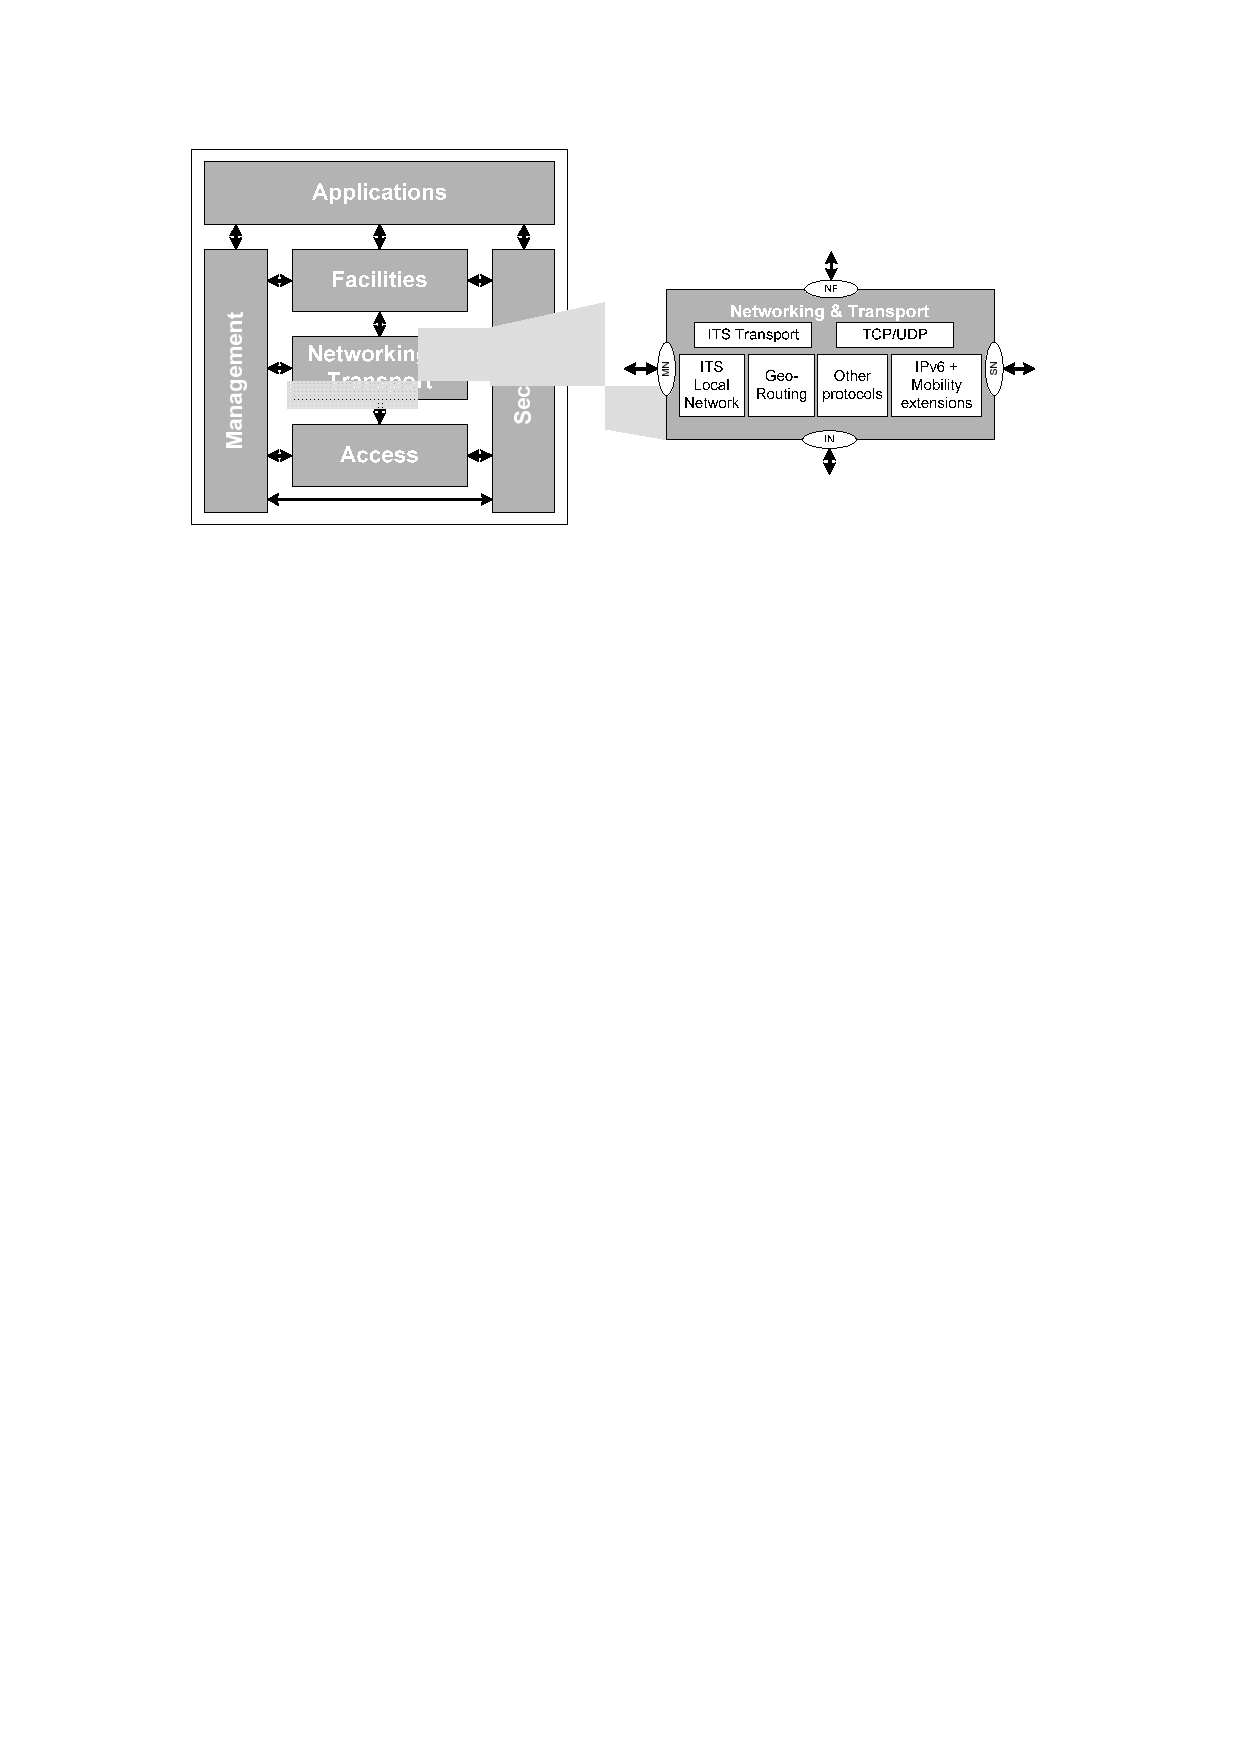
\includegraphics[width=0.95\textwidth]{content/images/03_networklayer/uebersichtLayer.pdf}
	\caption{Die Layer im Überblick mit Hervorhebung des Network Layers \cite{en302665}}
\label{fig:layerUeberblick-nwLayer}
\end{figure}


\subsection{Herausforderung}
Aufgrund der sich ständig ändernden Herausforderungen kommt es im \ac{C2C} Netz zu häufigen Paketverlusten und einem allgemeinen Overhead an Informationen. Die Änderungen bestehen darin, dass sich die Knoten mit sich ständig ändernden Geschwindigkeiten bewegen. Die Anzahl der Kommunikationspartner ist nicht konstant, sie ändert sich permanent. Neben der hohen Informationsdichte und Komplexität des Netzes muss eine Priorisierung der Nachrichten stattfinden können. Das Netz muss außerdem gewährleisten, dass die \ac{IVS} wissen, wie sie die umliegenden \ac{IVS} erreichen können.

\iffalse
Da sich die Topologie des C2C-Netzes ständig ändert, da die Knoten sich nicht nur mit unterschiedlichen Geschwindigkeiten bewegen sondern auch die Anzahl an Kommunikationspartnern sich dauernd ändert, kommt es in dem Netz zu häufigen Paketverlusten und einem allgemeinen Overhead an Informationen. Ausserdem muss gewährleistet werden das die einzelnen \ac{ITS-S} jederzeit wissen wie sie andere \ac{ITS-S} erreichen können. Zudem kommt noch hinzu das bei der hohen Informationsdichte und Komplexität des Netzwerkes noch unterschiedlich wichtige Nachrichten gesendet werden.
\fi

\subsection{Komponenten}
Im Folgenden werden die einzelnen Komponenten des Networklayers genauer erläutert. Zusätzlich wird darauf eingegangen, aus welchen Komponenten der Layer besteht, wie die einzelnen Komponenten arbeiten und welche Aufgaben sie erfüllen. Eine Übersicht über die Komponenten bietet die \autoref{fig:nwl}. 

\begin{figure}
	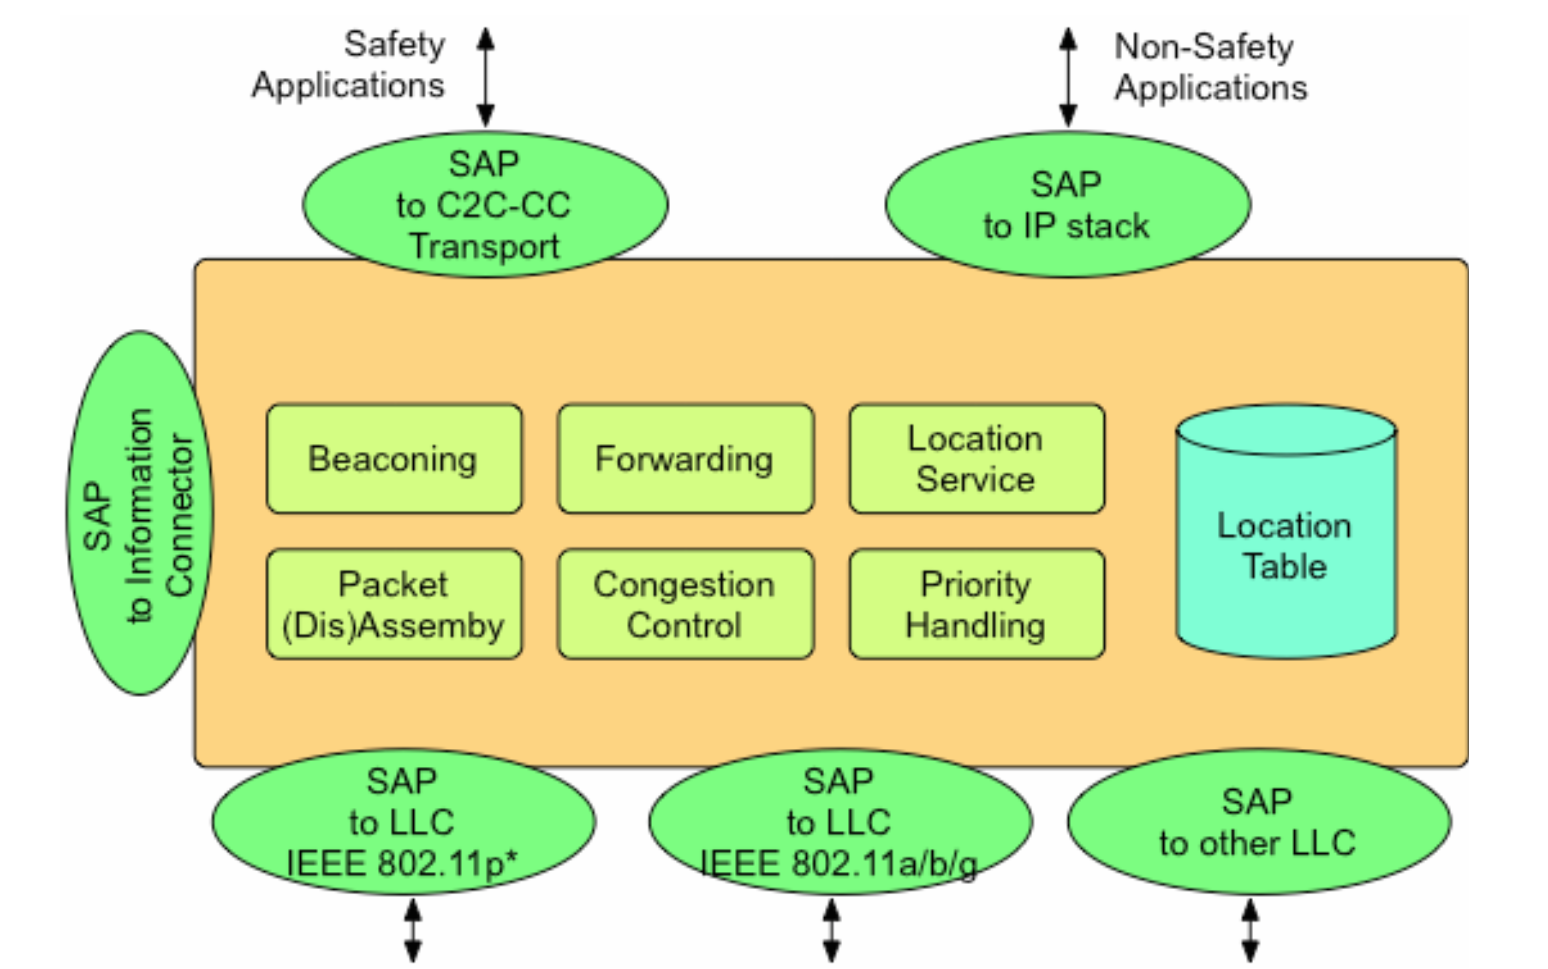
\includegraphics[width=0.99\textwidth]{content/images/03_networklayer/networklayer.png}
	\caption{Die Komponenten des Networklayers\cite{C2C-manifesto}}
	\label{fig:nwl}
\end{figure}

Wie auf \autoref{fig:layerUeberblick-nwLayer} zu sehen ist, hat der Network Layer Interfaces zum Access Layer (\autoref{subsec:accessLayer}), dem Management Layer (\autoref{architektur_managementLayer}), dem Security Layer (\autoref{architektur_securityLayer}) und dem Facilities Layer (\autoref{architektur_facilitiesLayer}).

\subsubsection{Location Table}
Jedes \ac{ITS-S} verfügt über eine Location Table. In dieser Tabelle werden Informationen über die naheliegenden Knoten, also \ac{ITS-S}, gespeichert. Diese Tabelle ist für das Forwarding notwendig, da hier unter anderem die Adressen und Positionen der zu erreichenden \ac{ITS-S} gespeichert sind. 
Im Folgenden werden einige der Informationen, die in einer solchen Tabelle enthalten sind, aufgeführt. Zusätzlich können dort noch weitere Informationen  gespeichert werden. Das genaue Format der Datensätze ist noch nicht spezifiziert und kann somit von diesem Dokument abweichen. Die Daten, die in der Location Table gespeichert sind, sind nur zeitweise korrekt, daher sind sie mit einem Timestamp versehen und werden nach einer gewissen Zeit verworfen. Die Informationen des Positionsvektors sollten mindestens über die unten aufgeführten Informationen verfügen. 
\begin{enumerate}
      \item C2C Netzwerkadresse
      \item MAC Adresse
      \item IPv6 Adresse
      \item Positionsvektor
      \begin{enumerate}
      	\item Geschwindigkeit
	\item Heading
	\item Geo. Position
	\item Zeitstempel des Vektors
	\item Genauigkeit des Vektors
      \end{enumerate}
      \item Version des Protokolls
      \item Typ des \ac{ITS-S}s
      \item Zeitstempel des zuletzt erhaltenen Paketes
      \item Datenrate des ITS
      \item Direkter Nachbar Flag
\end{enumerate}

\subsubsection{Beaconing}
Um die Informationen in der Location Table zu füllen, sendet jedes \ac{ITS-S} in einem periodischen Abstand eine sogenannte Beacon-Nachricht an seine Umgebung. In dieser Nachricht sind die oben aufgeführten Informationen enthalten. Jede \ac{ITS-S}, die diese Nachrichten empfängt aktualisiert bei Bedarf ihre Location Table.

\subsubsection{Forwarding}
Der Networklayer untersützt verschiedene Arten von Forwarding Algorithmen. Diese werden im späteren \autoref{sec:georouting} genauer erläutert.

\subsubsection{Location Service}
Es kann vorkommen, dass die Location Table leer ist, aber dennoch  eine Nachricht gesendet werden muss. In diesem Fall muss eine Weiterleitungsmöglichkeit gesucht werden. Diese Funktion bietet der Location Service. 
Über diesen können explizit Informationen zu einem Knoten, der die Nachricht weiterleiten kann, angefragt werden. Im Vergleich zu den Beacon-Nachrichten ist der Location Service ein On-Demand Dienst, der für Routenaufbau zuständig ist.

\begin{figure}
	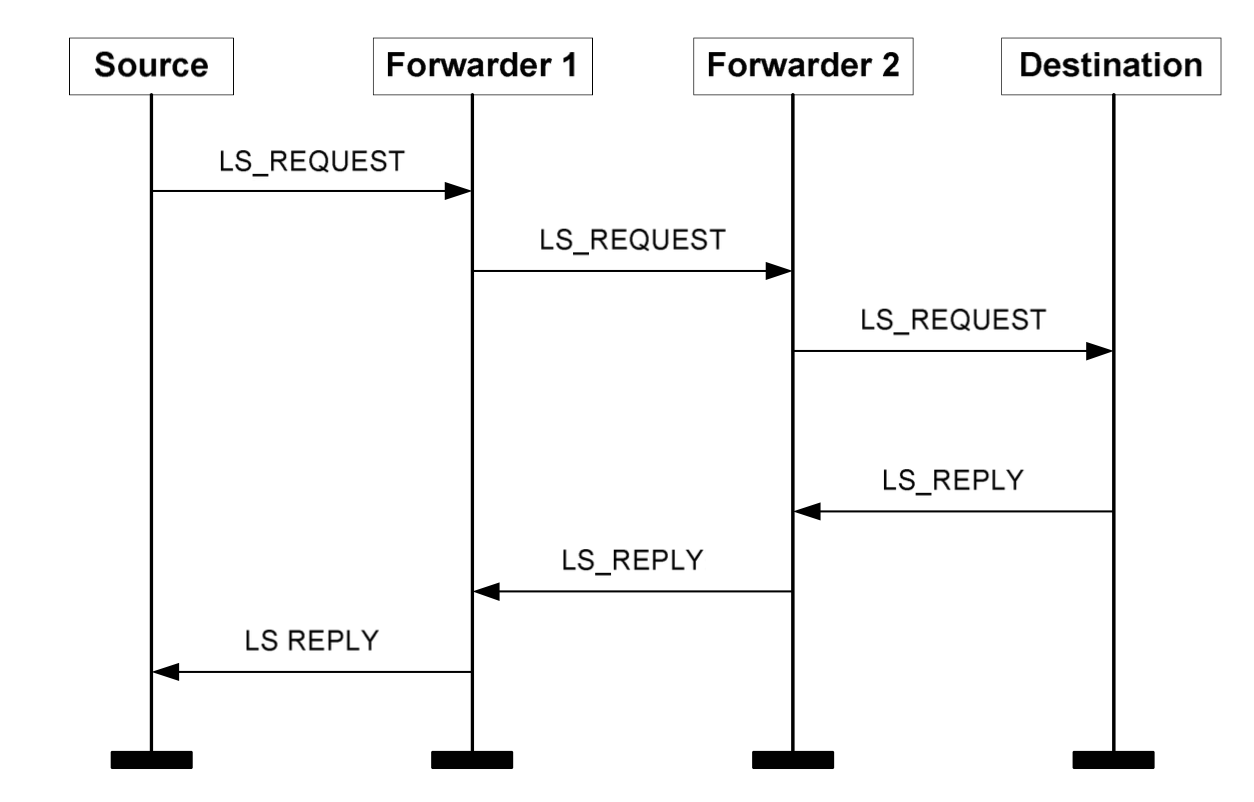
\includegraphics[width=0.99\textwidth]{content/images/03_networklayer/location-service-diagramm.jpg}
	\caption{Ablauf einer Anfrage des Location Service}
	\label{fig:locser}
\end{figure}

In \autoref{fig:locser} ist erkennbar, wie über den Location Service Informationen des Ziels über zwei Forwarding Knoten abgerufen werden. 

\subsubsection{Priority Handling}
Anhand der Paketpriorität wird entschieden, wie mit dem Paket verfahren wird. Hoch priorisierte Pakte werden vorrangig versendet. Um sicher zu stellen, dass die Pakte mit einer niedrigen Priorität dennoch ankommen, werden sie in eine Paketqueue eingereiht. 

%Damit wichtige Pakete zuerst gesendet werden können und andere dennoch empfangen werden, gibt es eine Paketqueue in die die unwichtigeren Nachrichten eingereiht werden. 

\subsubsection{Packet Assemby}
Da sich beim Versenden von Paketen die Positionsangaben der \ac{IVS}, sowie die Hops oder Time-to-Live ändern, muss der Networklayer dafür sorgen, dass die Pakete beim Weitersenden modifiziert oder aktualisiert werden. Hierfür werden die Informationen aus der Location Table verwendet.

\subsubsection{Congestion Control}
Die Congestion Control wird von \ac{DCC} (\autoref{architektur_dcc}) übernommen. Dadurch werden Paketstaus und Überläufe auch im Network Layer verhindert.

\iffalse
Da die Paketdichte in einem C2C-Netz sehr hoch werden kann und es zu Überläufen oder Paketstaus kommen kann, muss in extremen Situationen das Netz reguliert werden. \ac{ITS} sieht hierfür \ac{DCC} \autoref{architektur_dcc} vor. Es ist ein Mechanismus des Management Layers, muss aber um sinnvoll zu funktionieren in allen Layern vorhanden sein.  

 Hierauf wird in \autoref{sec:congestioncontrol} genauer eingegangen.
\fi

\section{Geo Routing\label{sec:georouting}}
Damit in \ac{C2C} die richtigen Routen gefunden werden können und die Ziele adressierbar sind, benötigen die Teilnehmer einmalige Adressen. Diese sind als \acl{GNW} Adresse spezifiziert. 

\subsection{Adressierung} 
Die \acl{GNW} Adresse besteht aus acht Bytes, welche verschiedene Informationen repräsentieren. Die ersten zwei Bytes zeigen, ob die Adresse manuell oder automatisch konfiguriert wurde, spezifizieren die \ac{ITS-S} und geben den den ITS-S Country Code an. Die restlichen sechs Bytes repräsentieren die MAC Adresse.\cite{etsi302636-4-1}

\begin{figure}
	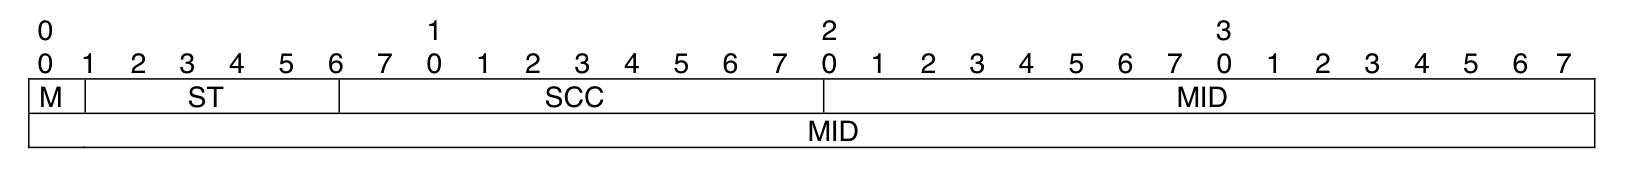
\includegraphics[width=0.99\textwidth]{content/images/03_networklayer/gnwadress.jpg}
	\caption{Format der \acl{GNW} Adresse}
	\label{fig:formatgnwa}
\end{figure}
Die auf der \autoref{fig:formatgnwa} zu sehenden Felder sind in der nachfolgenden \autoref{tab:formatgnwa} noch einmal genauer erläutert.

\begin{table}[h]
\begin{tabular}{llp{0.7\linewidth}}
\textbf{Feld} & \textbf{Feldname} & \textbf{Bedeutung} \\ \hline
    1 & M       & wird auf 1 gesetzt wenn die Adresse manuell vergeben worden ist, andernfalls auf 0          \\
    2 & ST    & Identifiziert um was es sich für eine ITS handelt       \\
    3 & SCC   &   ITS-S Country Code        \\
    4 & MID    &    erster Teil der MAC-Adresse       \\
    5 & MID     &   zweiter Teil der MAC-Adresse        \\
\end{tabular}
\caption{Felder und Bedeutung der \acs{GNW} Adresse \cite{etsi302636-4-1}}
\label{tab:formatgnwa}
\end{table}

Für das zweite Feld ST sind folgende Werte in \autoref{tab:typenspezi} spezifiziert.

\begin{table}[h]
\begin{tabular}{lll}
\textbf{Nummer} & \textbf{Bedeutung}  \\ \hline
    0 & Unknown \\
    1 & Pedestrian \\
    2 & Cyclist \\
    3 & Moped \\
    4 & Motorcycle \\
    5 & Passenger Car \\
    6 & Bus \\
    7 & Light Truck \\
    8 & Heavy Truck \\
    9 & Trailer \\
    10 & Special Vehicle \\
    11 & Tram \\
    15 & Road Side Unit \\
\end{tabular}
\caption{Werte für Feld zwei der \acs{GNW} Adresse \cite{etsi302636-4-1}}
\label{tab:typenspezi}
\end{table}

 \begin{itemize}
      	\item Geschwindigkeit
	\item Heading
	\item Geo. Position
	\item Zeitstempel des Vektors
	\item Genauigkeit des Vektors
\end{itemize}

\subsubsection{Konfiguration der Adressen}
Es gibt drei Vorgehensweisen, um eine \acl{GNW} Adresse zu konfigurieren.

\begin{enumerate}
      	\item Auto-address configuration
	\item Managed address configuration
	\item Anonymous address configuration
\end{enumerate}

Für die beiden ersten Verfahren ist das Duplicate address detection Verfahren vorgesehen. Es verhindert, dass \ac{ITS-S} Adressen mehrfach vorkommen.
Bei dem ersten Verfahren wird die Adresse automatisch von der \ac{ITS-S} generiert und sollte im Nachhinein nur bei einer duplicate address detection geändert werden. 

Managed address configuration stellt eine Anfrage an die ITS Networkung \& Transport Layer Management entity um seine Adresse zu konfigurieren. Hier darf die Adresse erneut von der \ac{ITS-S} angefordert werden oder die ITS Networkung \& Transport Layer Management entity sendet dieser eine Neue. Das anonyme Verfahren erlaubt es der \ac{ITS-S} eine anonyme Adresse zu konfigurieren, die von einer Sicherheitseinheit kontrolliert wird. Das anonyme Verfahren dient dem Datenschutz. Eine genaue Erklärung befindet sich in Trust and Privacy Manageement. 

\subsubsection{Duplicate address detection}
Die duplicate address detection kommt zum Einsatz, um zu gewährleisten, dass die \acl{GNW} Adresse tatsächlich einzigartig ist. Sobald ein Empfänger eine Nachricht erhält, vergleicht er seine eigene \acl{GNW} Adresse mit der des Paketes und danach die beiden MAC Adressen. Bei Übereinstimmung fordert er eine neue MAC-Adresse an und teilt dem System mit, dass eine doppelte Adresse entdeckt wurde. \cite{etsi302636-4-1}

\subsection{Geo Unicast}
Geo Unicast wird spezifiziert, um einen einzelnen Knoten zu adressieren. Die \ac{ITS-S}, die zwischen dem Sender und der Empfangseinheit liegen, dienen beim Senden als Zwischenstationen. Bei einem Geo Unicast kann eine Nachricht direkt, oder über mehrere Zwischenstationen, an die Ziel \ac{ITS-S} gesendet werden. Jede Zwischenstation entspricht dabei einem Hop. Sie dekrementiert den Hop Count der Nachricht um Eins und verwirft die Nachricht, wenn der Hop Count Null erreicht. Die Nachrichten können bei einem Hop verändert werden. Eine Veränderung kann in dem Fall eine Aggregation von mehreren Nachrichten zu Einer sein, oder das Aufteilen einer Nachricht zu Mehreren. Eine direkte Manipulation der Informationen, bzw. ein Hinzufügen von Informationen ist auch möglich.

%Die Nachricht kann bei den Zwischenstationen verändert werden. Das heisst zwei oder mehr Nachrichten werden zu einer zusammengefasst bevor sie weitergesendet werden. Dieser Vorgang ist auch umgekehrt durchführbar, sodass eine Nachricht aufgeteilt werden kann. Der Inhalt der Nachricht kann ebenfalls verändert oder Informationen hinzugefügt werden. 

\begin{figure}
	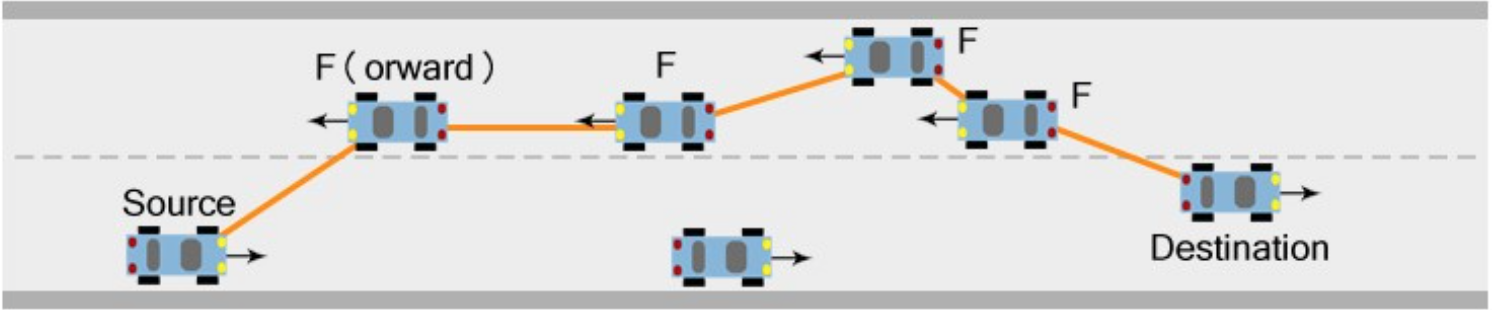
\includegraphics[width=0.99\textwidth]{content/images/03_networklayer/GeoUnicast.png}
	\caption{Geo Unicast \cite{etsi102636-1}}
	\label{fig:geounicast}
\end{figure}

\subsection{Topologically-scoped broadcast}
Der Topologically-scoped broadcast sendet eine Nachricht mit einem bestimmten Hop Count an alle, direkt vom  Knoten erreichbaren, Einheiten. Diese Nachricht wird dann von den Knoten empfangen, bei denen der Hop Count endet.

\begin{figure}
	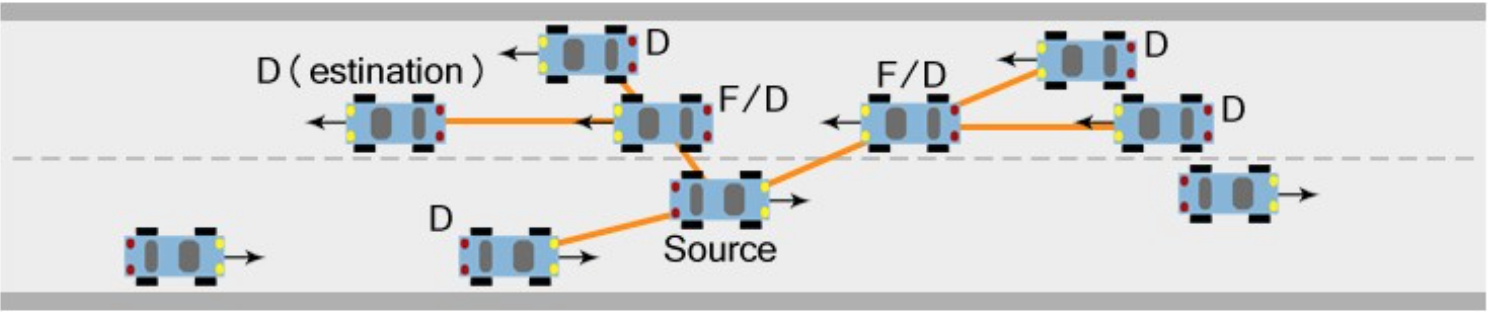
\includegraphics[width=0.99\textwidth]{content/images/03_networklayer/TSC.png}
	\caption{Topologically-scoped broadcast mit Hop Count 2 \cite{etsi102636-1}}
	\label{fig:tsc}
\end{figure}


\subsection{Geographically-scoped broadcast}
Über den Geographically-scoped broadcast ist es einem Knoten möglich, eine bestimmte Region, die sich um ihn herum befindet, zu erreichen. Die Region wird durch den Standort der \ac{ITS-S} und einen Radius definiert. Dabei spielt die Anzahl der Hops keine Rolle, alle \ac{ITS-S}, die sich in dieser Region befinden, sind adressiert.

\begin{figure}
	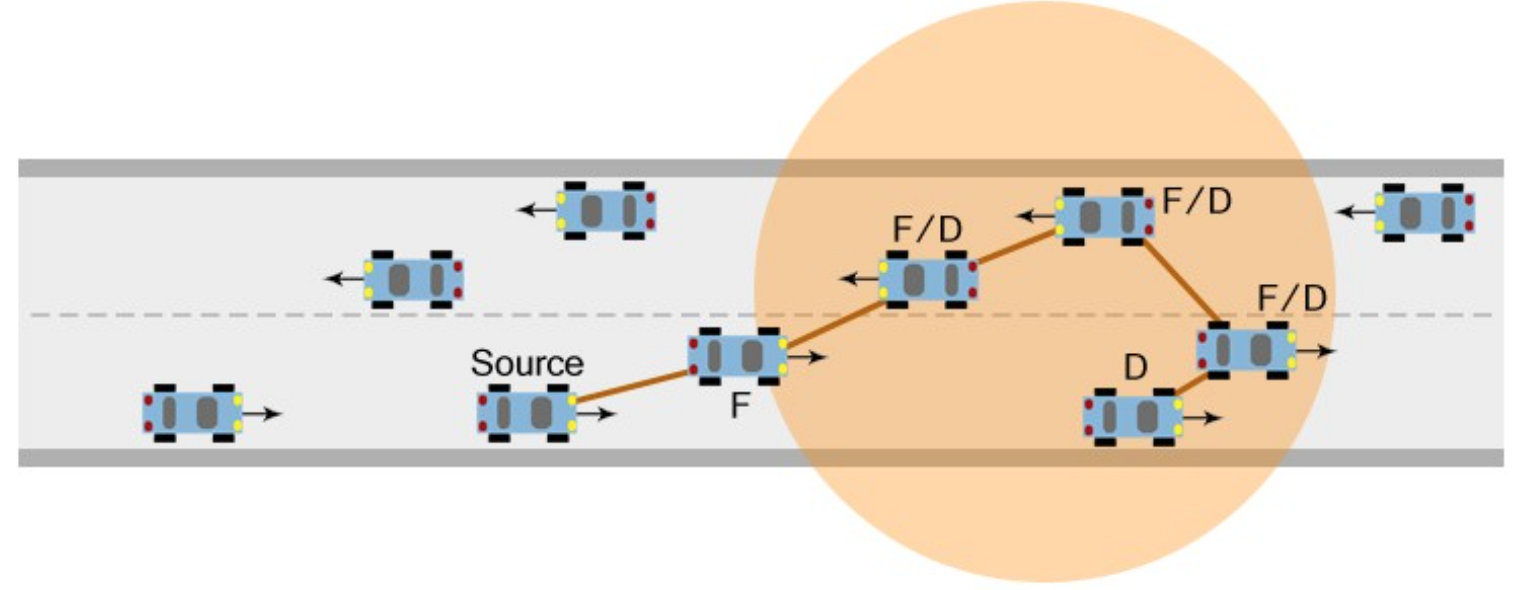
\includegraphics[width=0.99\textwidth]{content/images/03_networklayer/GSB.png}
	\caption{geographically-scoped broadcast \cite{etsi102636-1}}
	\label{fig:gsb}
\end{figure}

\subsection{Geographical Scoped Anycast}
Der Geographical Scoped Anycast ist ähnlich zu dem Geographically-scoped broadcast. Der Unterschied ist, dass hier die Nachricht innerhalb der Region nicht weitergeleitet wird. Das Routing stoppt, sobald ein Ziel innerhalb der Region die Nachricht empfangen hat.

\begin{figure}
	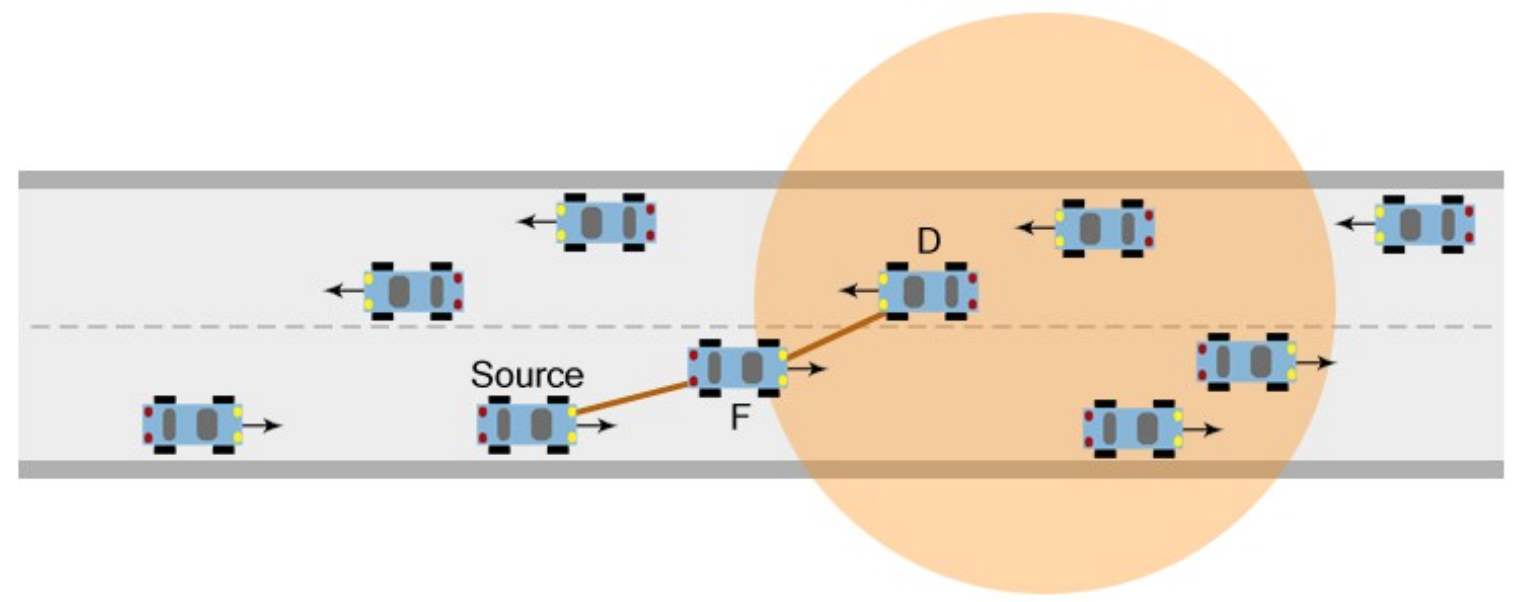
\includegraphics[width=0.99\textwidth]{content/images/03_networklayer/GSA.png}
	\caption{geographically-scoped anycast \cite{etsi102636-1}}
	\label{fig:gsa}
\end{figure}

